\documentclass{book}
\usepackage{mathalpha}
\usepackage[utf8]{inputenc}
\usepackage{cancel}
\usepackage[margin=2cm, a4paper]{geometry}
\usepackage{amsmath}
\usepackage{amssymb}
\usepackage{gensymb}
\usepackage{graphicx}
\usepackage{hyperref}
\usepackage{pgfplots}
\usepackage{tikz}
\usepackage{pdfpages}
\usepackage{parskip}
\usepackage{polynom}
\usepackage{multirow}

\newenvironment{generalInformation}{}{}
\newenvironment{explanationOfTerms}{}{}
\newenvironment{example}{}{}
\newenvironemnt{note}{\begin{center}\em NOTE: }{\end{center}}

\title{Physics}
\author{Lachlan Takumi Ikeguchi}

\begin{document}
\maketitle
\tableofcontents

\section{The purpose}
This document was written to be used as a summary to help revise the content covered in Physics.  For any inquiries, feedback, and further explanations, contact lachlanprivate@duck.com or through the discord server: \url{https://discord.gg/6P8rddkXFr}.  I encourage you to let me know of any topic I missed, how I could explain it better, or how it could be reworded or formatted to be more helpful in its purpose.  The goal of this document is to be a comprehensive summary of everything you need to know.

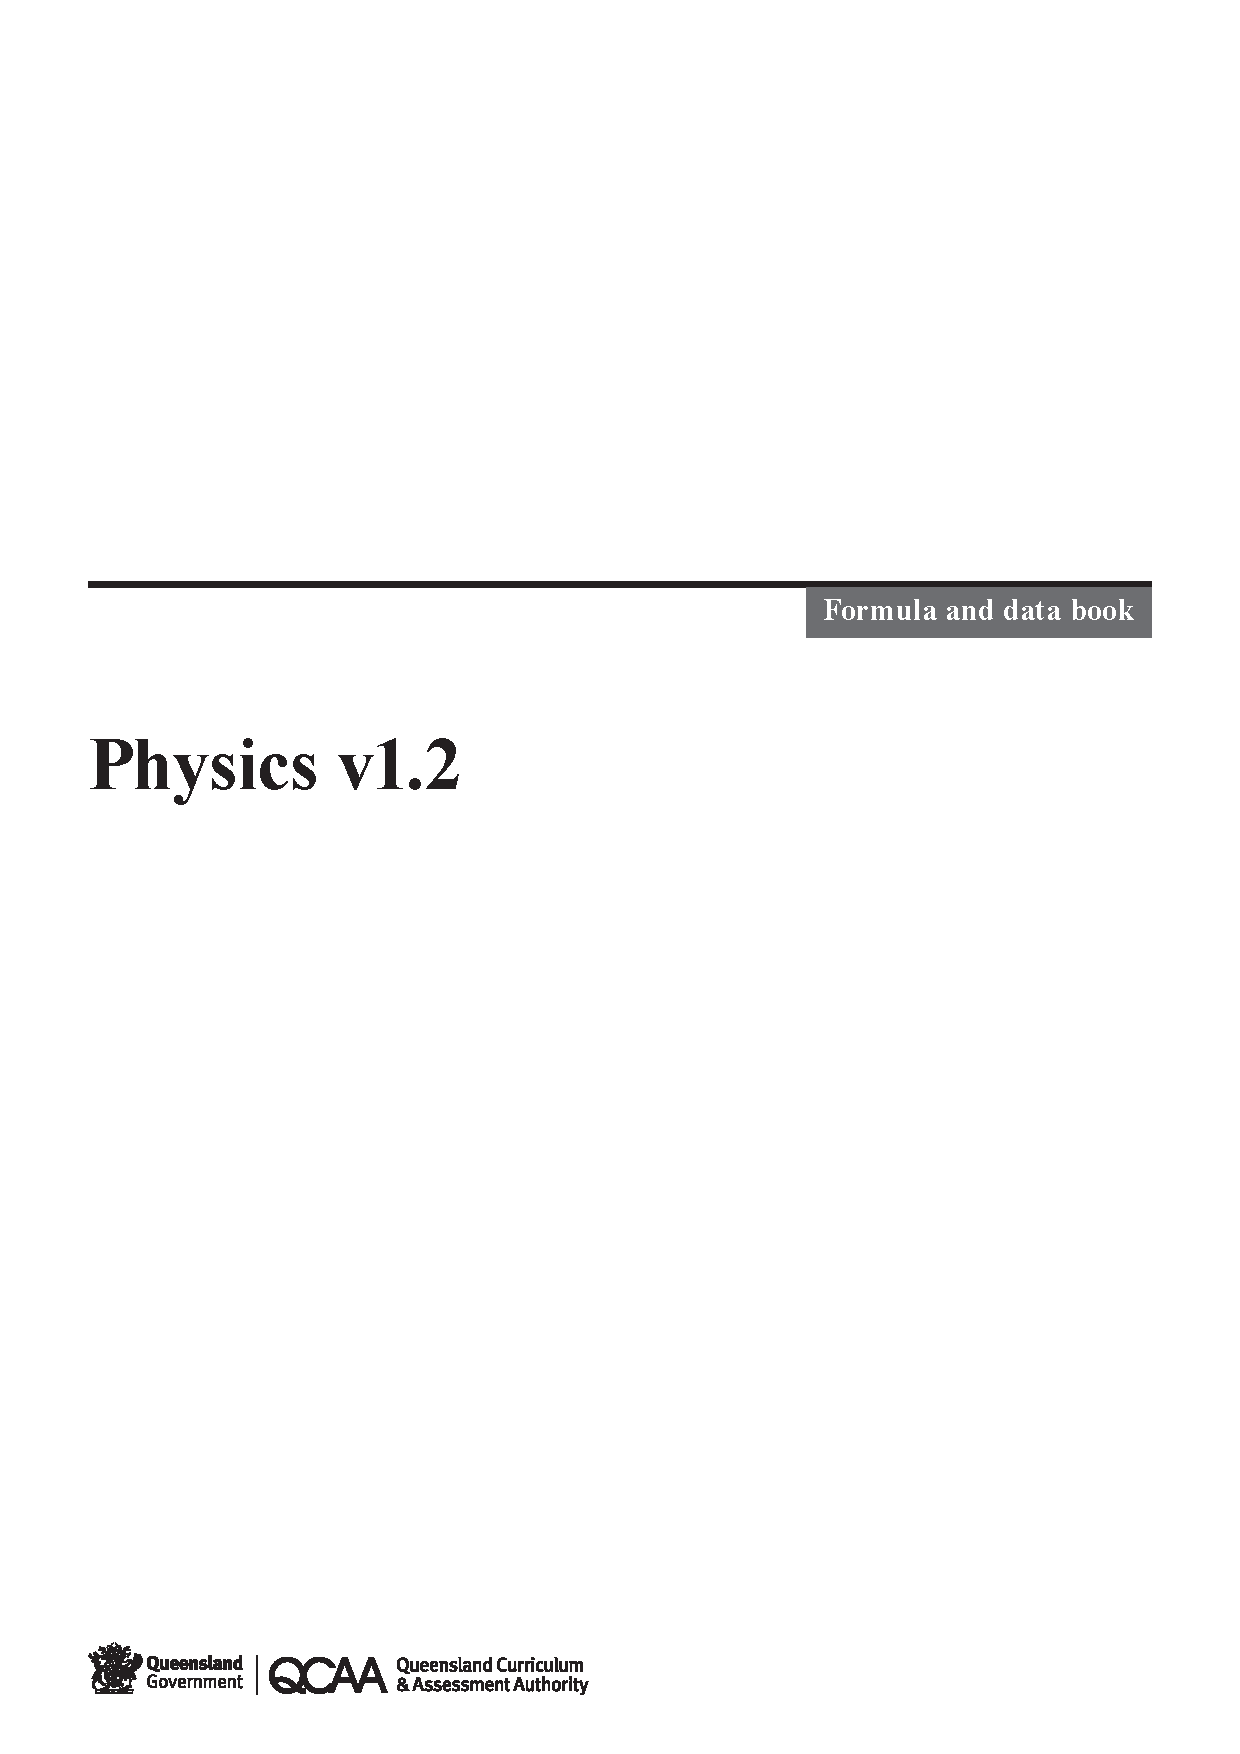
\includepdf[pages={1-9}]{./images/formula-book.pdf}

\chapter{Data}
\section{Measurement uncertainty}

\section{Error}



\chapter{Heating process}
\section{Kinetic particle model}
\begin{generalInformation}
    The kinetic particle model states that all matter are made of particles that are in constant motion.
\end{generalInformation}


\section{Internal energy}
\begin{generalInformation}
    Internal energy is the energy that the object contains.  Internal energy is donated the letter $U$ and is measured in Joules.  There are two classifications of internal energy, macroscopic, and microscopic.
\end{generalInformation}
\subsection{Macroscopic}
\begin{generalInformation}
    Macroscopic internal energy is the energy of the object as a whole.

    This includes:
    \begin{itemize}
        \item Kinetic energy
        \item Gravitational potential energy
    \end{itemize}
\end{generalInformation}

\subsection{Microscopic}
\begin{generalInformation}
    Microscopic internal energy is the energy of the particles that make up the object.

    This includes:
    \begin{itemize}
        \item Thermal energy
        \item Chemical potential energy
        \item Nuclear energy
    \end{itemize}
\end{generalInformation}


\section{Temperature}
\begin{generalInformation}
    Temperature is the average kinetic energy of the particles of an object.  It is donated the letter $T$ and is measured in Kelvins, Celsius, or Fahrenheit.
\end{generalInformation}

\section{Heat}
\begin{generalInformation}
    Heat is defined as the rate of transfer of internal energy.  
\end{generalInformation}


\section{Specific heat capacity}


\section{Calorimetry}


\section{Specific latent heat}



\chapter{Radiation and nuclear reactions}
\section{Nuclear model}


\section{Mass defect and binding energy}


\section{Nuclear decay}


\section{Half-life}


\section{Fission}


\section{Fusion}



\chapter{Electrical circuits}
\section{Charge}


\section{Current}


\section{Voltage}


\section{Power}


\section{Resistance}
\subsection{Series}

\subsection{Parell}

\section{Kirchhoff's Laws}

\section{Circuit analysis}



\chapter{Linear motion}
\section{Scalar quantities}
\subsection{Speed}

\subsection{Distance}


\section{Vector quantities}
\subsection{Velocity}

\subsection{Displacement}

\subsection{Acceleration}


\section{Newton's laws}
\subsection{1st law}

\subsection{2nd law}

\subsection{3rd law}


\section{Equations of motion}
\subsection{Motion due to gravity}


\section{Momentum}


\section{Collisions}
\subsection{Elastic}

\subsection{Inelastic}


\section{Work}


\section{Energy}
\subsection{Kinetic energy}

\subsection{Gravitational potential energy}



\chapter{Waves and Light}
\section{Characteristics}


\section{Transverse}


\section{Longitudinal}


\section{Reflection}


\section{Refraction}
\subsection{Lenses}

\subsetion{Total internal reflection}


\section{Diffraction}


\section{Polarization}

\end{document}
